\documentclass[10pt]{report}
\usepackage[utf8]{inputenc}
\usepackage{amsfonts}
\usepackage{amsmath}
\usepackage{amssymb}
\usepackage{commath}
\usepackage[ngerman]{babel}
\usepackage{enumitem}
\usepackage{booktabs}
\usepackage{longtable}
\usepackage{relsize}
\usepackage{pgfplots}
\usepackage{csvsimple}
\usepackage{pgfplotstable}
\usepackage{siunitx} % Formats the units and values
\usepackage{fancyhdr}
\usepackage{float}



\pagestyle{fancy}
\fancyhf{}
\lhead{GPET Versuch 1}
\rhead{Tim Luchterhand, Paul Nykiel}
\cfoot{\thepage}

\setcounter{chapter}{8}

\setlength\parindent{0pt}

\author{Tim Luchterhand, Paul Nykiel}
\title{GPET Versuch 1}

\begin{document}
        \maketitle
        \section{Messwerte mit Python}
        Leider wurde das Multimeter am Computer nicht erkannt.

        \section{Widerstandskennlinie}
        \subsection{Leistung}
        \begin{eqnarray*}
            I = \frac{U_{max}}{R} = \frac{30V}{220k \Omega} &=& 0.136 mA\\
            P = \frac{U_{max}^2}{R} &=& 4.1 mW
        \end{eqnarray*}
        \noindent Die maximale Leistung, die der Widerstand aufnimmt, liegt deutlich
        unter der kritischen Schranke. Es besteht also keine Gefahr für den Widerstand,
        selbst bei einer maximalen Spannung von 30V.
        \subsection{Messwerte}

        \begin{table}[H]
            \begin{center}
                \caption{Messwerte für Stromfehlerschaltung}
                \label{table1}
                \pgfplotstabletypeset[
                multicolumn names, % allows to have multicolumn names
                col sep=space, % the seperator in our .csv file
                display columns/0/.style={
                column name=$U_B$, % name of first column
                column type={S},string type},  % use siunitx for formatting
                display columns/1/.style={
                column name=$U_x$,
                column type={S},string type},
                display columns/2/.style={
                column name=$I$,
                column type={S},string type},
                display columns/3/.style={
                column name=$R_x$,
                column type={S},string type},
                display columns/4/.style={
                column name=$\Delta R$,
                column type={S},string type},
                display columns/5/.style={
                column name=$\rho_R$,
                column type={S},string type},
                every head row/.style={
                before row={\toprule}, % have a rule at top
                after row={
                \si{\volt} & \si{\volt} & $\mu$\si{\ampere} & k\si{\ohm} & k\si{\ohm} & \%\\
                \midrule} % rule under units
                },
                every last row/.style={after row=\bottomrule},
                ]{widerstandskennlinie.csv}
            \end{center}
        \end{table}

        \vspace{0.5cm}

        \textbf{Messungenauigkeit:} $0.5\% + 2$

        \textbf{Innenwiderstand:} 11.18M$\Omega$ bei 5V,
                10.1M$\Omega$ bei den anderen Messungen


        \subsection{Auswertung}
        Die Messwerte sind für die Spannungen größer 5V fast identisch,
        für Werte kleiner 6V ist der Innenwiderstand des Messgeräts höher.
        Der ermittelte Widerstandswert weicht ebenfalls deutlich von den anderen Messungen ab.

        Die vereinfachte Formel lässt sich nur verwenden, wenn der Innenwiderstand
        des Spannungsmessgeräts deutlich größer ist, als der zu messende Widerstand.
        Beim digitalen Messgerät gibt es keine feste Innenimpedanz, weshalb die
        ausführliche Formel verwendet wurde.

        \subsection{U-I-Diagram}
        \begin{center}
            \begin{tikzpicture}
        		\begin{axis}[ymin=0, xlabel = {V}, ylabel = {$\mu$ A}]
        			\addplot table[x index = {1},
                            y index = {2}] {widerstandskennlinie.csv};
        		\end{axis}
        	\end{tikzpicture}
        \end{center}

        \noindent Das Diagram zeigt eine Gerade mit Steigung R. Die Kurve hätte ein Offset am
        Schnittpunkt mit der y-Achse, dieser ist der Messungenauigkeit bei 5V
        geschuldet.

        \section{Oszilloskop}
        \begin{figure}[H]
         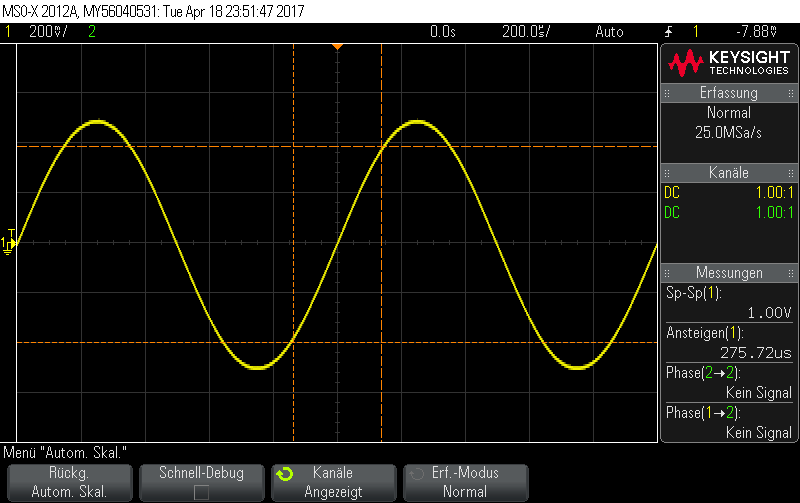
\includegraphics[width=\textwidth]{scope_13.png}
         \caption{Frequenzmessung}
       \end{figure}
        Nach Betrachtung der Skalierung erkennt man das eine Periode genau 5 Blöcke
        mit jeweils $2 \mu$s dauert, die Frequenz ist also 1kHz, wie eingestellt.

        Wie im Bild zu erkennen, beträgt die Spitze-Spitze Spannung $1$V,
        genau wie eingestellt (siehe Sp-Sp Wert unter Messungen).


       \subsection{Trigger}

        Der Anfang der Messung ist an dem Punkt, an dem der Trigger zum ersten mal
        ausgelöst wird. Somit verschiebt sich das Bild lediglich horizontal, wenn
        man das Trigger Level ändert.

         \noindent Sobald das Trigger Level höher bzw.\ niedriger als das Signal eingestellt ist,
         wird der Trigger nicht ausgelöst, es wird also nicht gemessen. Man kann kein sinnvolles
         Signal erkennen.

         \section{DC-AC Einstellung}
         \begin{figure}[H]
          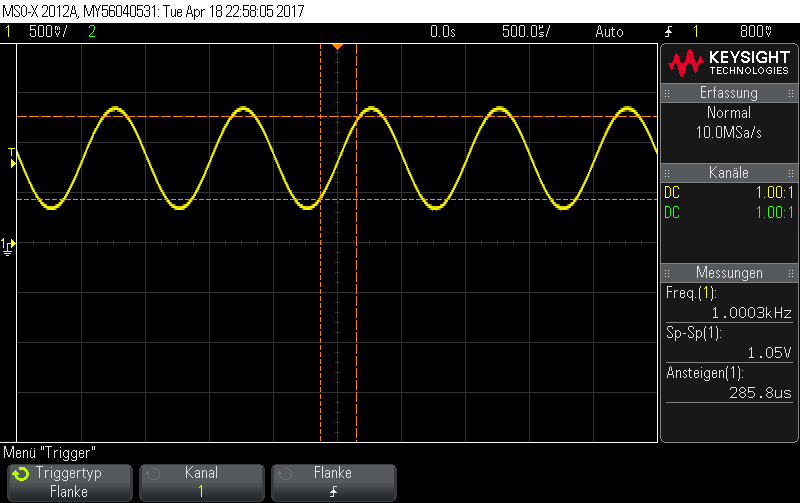
\includegraphics[width=\textwidth]{scope_6.png}
          \caption{DC: Das Signal ist um das eingestellte Offset verschoben}
        \end{figure}

         \begin{figure}[H]
          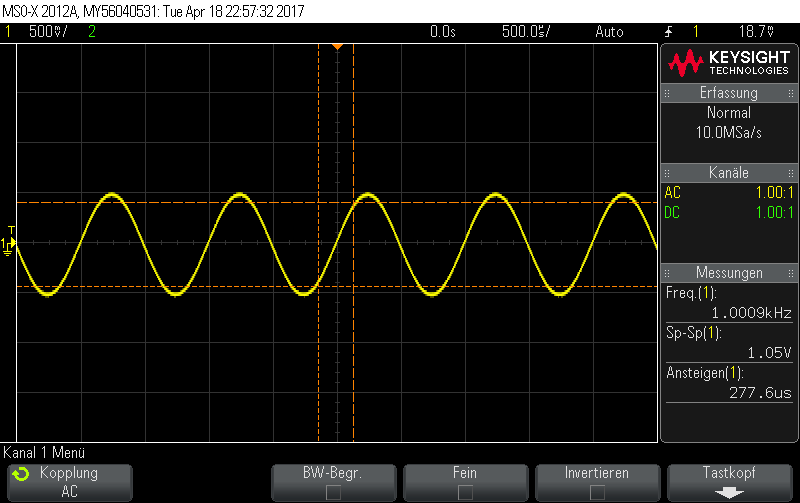
\includegraphics[width=\textwidth]{scope_5.png}
          \caption{AC: Das Signal wird ohne Verschiebung angezeigt, da Gleichanteile heraus
          gefiltert werden}
        \end{figure}

         \noindent \textbf{Signalverzerrung:} Das verwendete Rechtecksignal hat eine Amplitude von 1 Volt Spitze-
         Spitze und eine Frequenz von 100 Hz.
         \begin{figure}[H]
          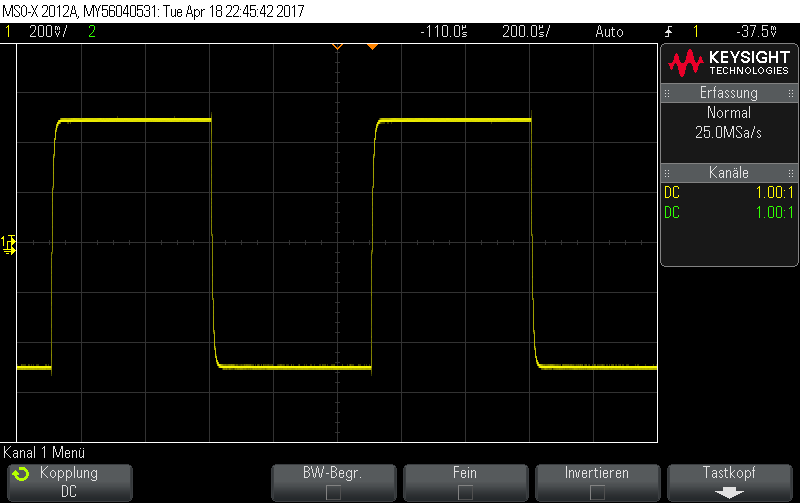
\includegraphics[width=\textwidth]{scope_1.png}
          \caption{Signalverzerrung}
        \end{figure}

         \noindent \textbf{Beobachtung:} Durch den Koppelkondensator erscheint
         das Rechtecksignal nicht mehr scharf,
         sonder besitzt abgerundete Flanken.

         \section{Kondensatormessung}
         Die Anstiegszeit $\Delta x$ wird mit dem Oszilloskop gemessen,
         daraus lässt sich die Zeitkonstant $\tau$ bestimmen. Durch
         die Beziehung $\tau = R \cdot C$ lässt sich die Kapazität
         bestimmen.
         \begin{figure}[H]
          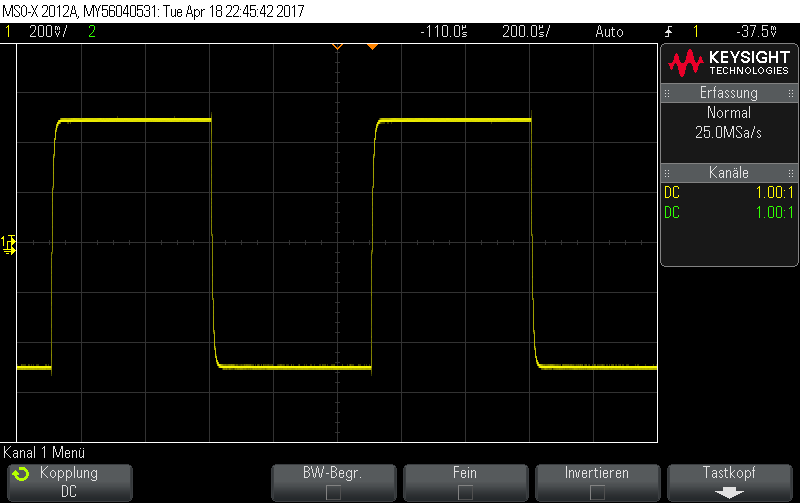
\includegraphics[width=\textwidth]{scope_1.png}
          \caption{Signal}
        \end{figure}

        \subsection{Messergebnisse mit Cursor}
        \begin{eqnarray*}
            \Delta x = 24 \mu s &\Rightarrow& \tau =  11 \mu s \\
            \tau = RC &\Rightarrow& C = \frac{\tau}{R}\\
            &\Rightarrow& C=218\text{nF}
        \end{eqnarray*}
        \begin{figure}[H]
         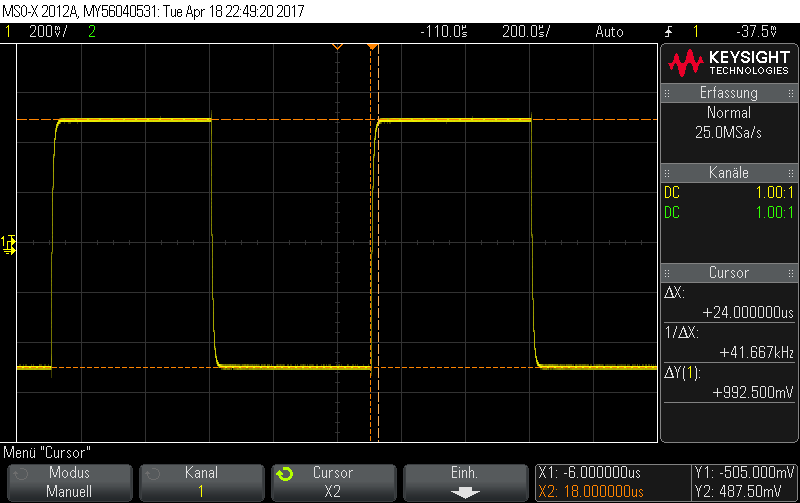
\includegraphics[width=\textwidth]{scope_2.png}
         \caption{Messung mit Cursor}
       \end{figure}

       \subsection{Messergebnisse mit Measure}
       \begin{eqnarray*}
           \Delta x = 9,74 \mu s &\Rightarrow& \tau =  4,43 \mu s \\
           \tau = RC &\Rightarrow& C = \frac{\tau}{R}\\
           &\Rightarrow& C=88.5\text{nF}
       \end{eqnarray*}
       \begin{figure}[H]
        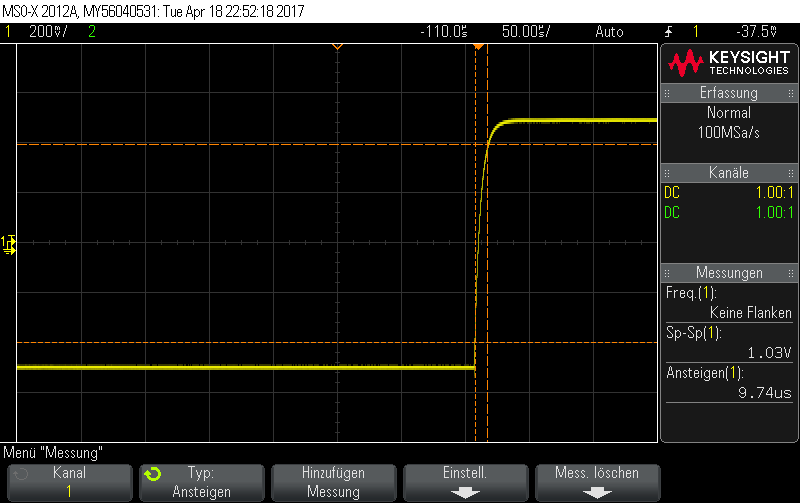
\includegraphics[width=\textwidth]{scope_4.png}
        \caption{Messung mit Measure}
      \end{figure}

      \subsection{Messergebnisse mit Multimeter}
      \begin{equation*}
          C = 97\text{nF}
      \end{equation*}

      \subsection{Abweichung}
      \subsubsection{Relativer Fehler zur Messung mit Multimeter}
      \begin{eqnarray*}
          \rho &=& \frac{\abs{C_{mess} - C_{multimeter}}}{C_{multimeter}}\\
          \\
          \rho_{Cursor} &=& 125\% \\
          \rho_{Measure} &=& 8.76\%
      \end{eqnarray*}

      \subsubsection{Fazit}
      Vor allem zwischen der Messung mit Cursor und den beiden anderen Messungen
      ist ein großer Unterschied zu vermerken. Das liegt vor allem daran, dass die
      Anstiegszeiten manuell bestimmt werden mussten und dementsprechend ungenau sind.
      Durch eine bessere Wahl des Bildausschnitts könnte eine deutlich genauere
      Messung mit manuellem Cursor erzielt werden.

      Die Messergebnisse der Messung mit Measure und Multimeter liegen deutlich
      näher beieinander, ein Wert der Kapazität des Kondesators zwischen
      $88.5$nF und $97$nF ist deshalb deutlich wahrscheinlicher.


      \section{Tiefpass}
      Die Grenzfrequenz lässt sich bestimmen durch Anpassen der Frequenz
      am Funktionsgenerator. Wenn das gefilterte Signal (in grün)
      eine Spitze-Spitze Spannung von $0.71$V ($\frac{1}{\sqrt{2}}$V) erreicht,
      beträgt die Grenzfrequenz die am Funktionsgenerator eingestellte Frequenz.

      \vspace{0.5cm}

      \textbf{Ermittelte Grenzfrequenz:} $1.9$kHz


      \begin{figure}[H]
       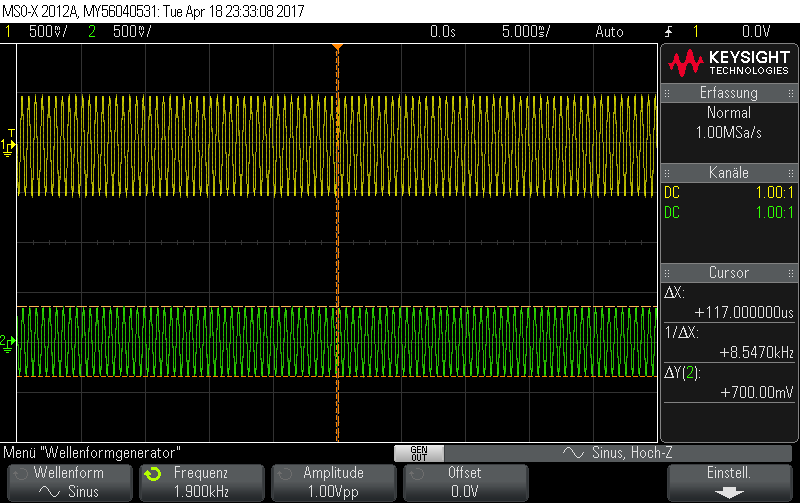
\includegraphics[width=\textwidth]{scope_8.png}
       \caption{Grenzfrequenz mit Cursor}
     \end{figure}

     Die Phasenverschiebung wurde durch die automatische Measure-Funktion des
     Oszilloskops bestimmt und beträgt $49^\circ$. Idealerweise sollte die
     Phasenverschiebung bei Grenzfrequenz genau $45^\circ$ betragen, eine
     Abweichung von $4^\circ$ ist also eher gering.

     \vspace{0.5cm}

     \textbf{Ermittelte Phasenverschiebung:} $49^\circ$
     \begin{figure}[H]
      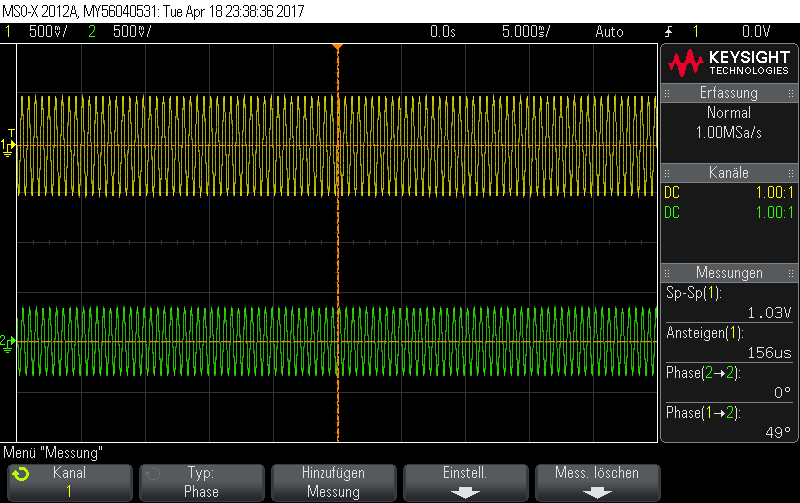
\includegraphics[width=\textwidth]{scope_9.png}
      \caption{Phasenverschiebung bei Grenzfrequenz}
    \end{figure}

    \section{Tastkopf}

    \begin{figure}[H]
     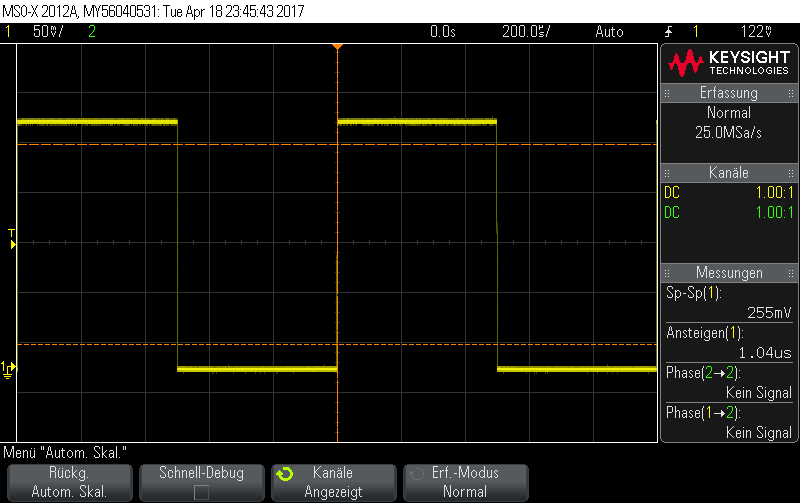
\includegraphics[width=\textwidth]{scope_12.png}
     \caption{Optimale Rechteckform: Bei einer optimalen Einstellung ist, wie im Bild zu sehen, kein Über- oder
     Unterschwingen zu erkennen. Die Spannungspeaks verlaufen genau parallel zur
     x-Achse.}
   \end{figure}


   \begin{figure}[H]
    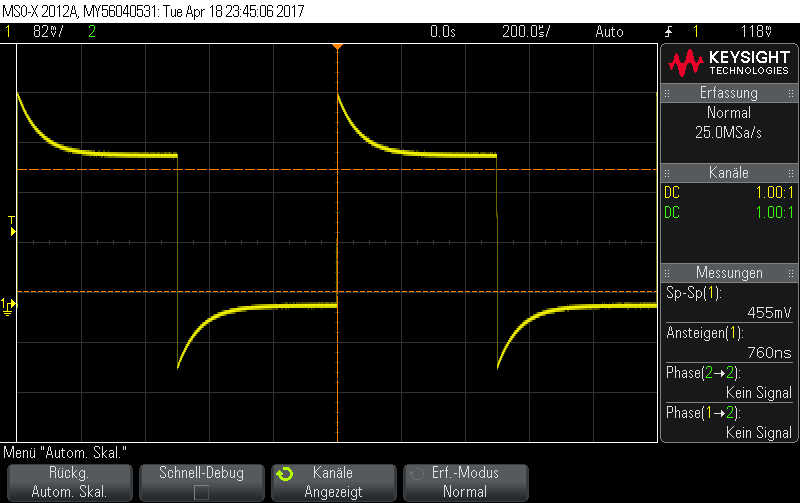
\includegraphics[width=\textwidth]{scope_11.png}
    \caption{Überschwingen: Zu Begin jedes Duty-Cycles schießt die Spannung kurz betragsmäßig über die
    eingestellte
    maximale Amplitude hinaus und fällt dann exponentiell ab bis die eingestellte
    Amplitude erreicht wird.}
  \end{figure}


  \begin{figure}[H]
   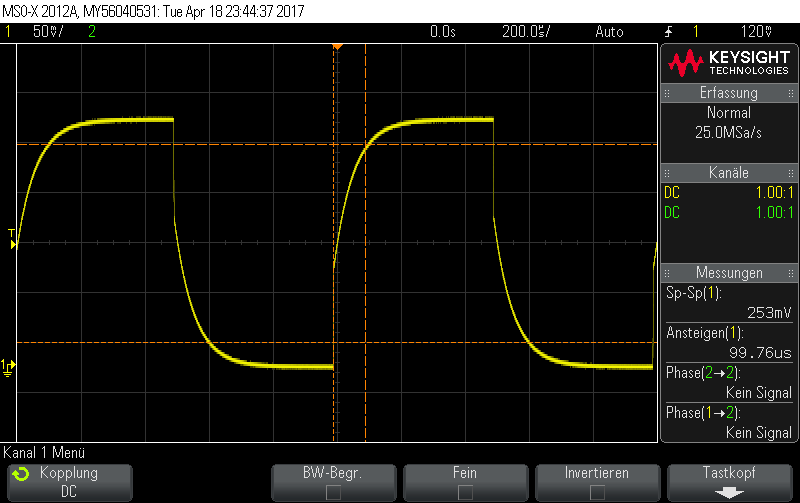
\includegraphics[width=\textwidth]{scope_10.png}
   \caption{Unterschwingen: Die Spannung liegt zu Begin jedes Duty-Cycles betragsmäßig unter der eingestellten
   Amplitude und steigt mit der Zeit erst auf diese an.}
 \end{figure}


\end{document}
